% Standalone export of Fig. 1 (exact-evaluation protocol). Kept in sync with main.tex.
\documentclass[border=2pt]{standalone}
\usepackage{amsmath,amssymb}
\usepackage{times}
\usepackage{tikz}
\usetikzlibrary{positioning,arrows.meta}
\begin{document}
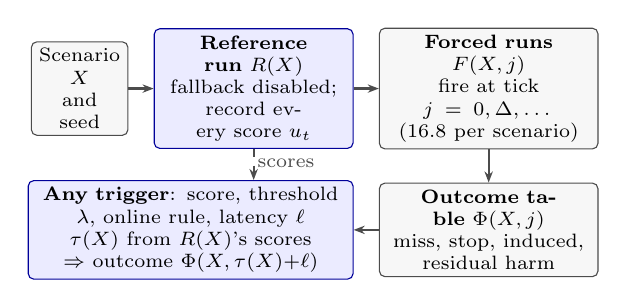
\begin{tikzpicture}[font=\scriptsize,
  box/.style={draw=black!70, rounded corners=2pt, align=center, inner sep=2.5pt,
              minimum height=0.95cm, fill=black!3},
  key/.style={box, fill=blue!8, draw=blue!60!black},
  arr/.style={-{Stealth[length=4pt]}, thick, black!70}]
\node[box, text width=1.05cm] (sc) {Scenario $X$\\ and seed};
\node[key, text width=2.35cm, right=0.32cm of sc] (ref)
  {\textbf{Reference run} $R(X)$\\ fallback disabled;\\ record every score $u_t$};
\node[box, text width=2.6cm, right=0.32cm of ref] (forced)
  {\textbf{Forced runs} $F(X,j)$\\ fire at tick $j = 0,\Delta,\dots$\\ (16.8 per scenario)};
\node[box, text width=2.6cm, below=0.42cm of forced] (table)
  {\textbf{Outcome table} $\Phi(X,j)$\\ miss, stop, induced,\\ residual harm};
\node[key, text width=3.95cm, left=0.32cm of table] (lookup)
  {\textbf{Any trigger}: score, threshold $\lambda$, online rule, latency $\ell$\\
   $\tau(X)$ from $R(X)$'s scores $\Rightarrow$ outcome $\Phi(X,\tau(X){+}\ell)$};
\draw[arr] (sc) -- (ref);
\draw[arr] (ref) -- (forced);
\draw[arr] (forced) -- (table);
\draw[arr] (table) -- (lookup);
\draw[arr, dashed] (ref.south) -- node[right, pos=0.45, inner sep=1pt] {scores} (ref.south |- lookup.north);
\end{tikzpicture}
\end{document}
